\documentclass[a4paper, 11pt]{article}

\usepackage[utf8]{inputenc}
\usepackage{graphicx}
\usepackage{amsmath}
\usepackage{amsfonts}
\usepackage{hyperref}
\usepackage{enumitem}
\usepackage{wrapfig}

\usepackage{tikz}
\usetikzlibrary{shapes,arrows,automata}

\title{M1 Project - Distributed Systems}
\author{Simon Mauras}

\begin{document}

\maketitle

\tableofcontents


\section{Introduction}

This report describe the implementation in Erlang of a small middle-ware using a treap topology. This project is part of the evaluation of a master's degree lecture at ENS Lyon.

After a first part in which explicit what a treap is, we are going to explain in detail the functionalities of our middle-ware. A third part will be devoted to give installation instructions. We will conclude by answering to the questions asked in the project assignment.

\newpage



\section{Treaps}

\subsection{Definitions}

The word treap is a portmanteau formed by the words tree and heap. The idea is to combine those two data-structures to build a new object having nice properties.

\medskip We recall that a Binary Search Tree (BST) is an indexed binary tree in which the value of each node is bigger than the values of the nodes of its left sub-tree and is lower than the values of the nodes of its right subtree. A heap is an indexed tree in which the value of each node is bigger than the values of its subtree.

\medskip If we combine those two kind of trees we can define a new data-structure in which each node is associated to a couple of values, the tree is a BST according to the first coordinate and a heap according to the second.

\begin{figure}[h!]
  \centering
  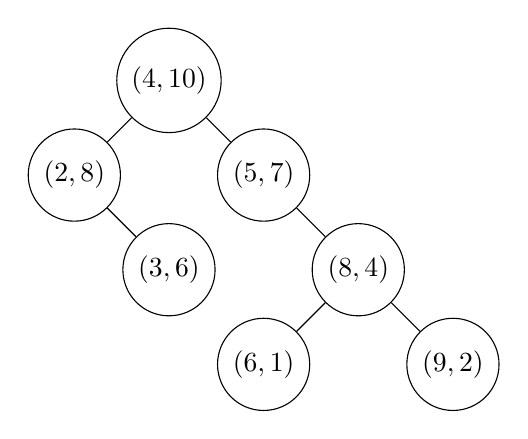
\begin{tikzpicture}[node distance = 1.7cm]
    \node[state] (A) {$(4, 10)$};
    \node[state] (B) [below left of=A] {$(2, 8)$};
    \node[state] (C) [below right of=B] {$(3, 6)$};
    \node[state] (D) [below right of=A] {$(5, 7)$};
    \node[state] (E) [below right of=D] {$(8, 4)$};
    \node[state] (F) [below left of=E] {$(6, 1)$};
    \node[state] (G) [below right of=E] {$(9, 2)$};
    \path (A) edge (B)
          (B) edge (C)
          (A) edge (D)
          (D) edge (E)
          (E) edge (F)
          (E) edge (G);
  \end{tikzpicture}
  \caption{Example of Treap.}
\end{figure}

We can notice that a treap is unique and can be build greedily. Indeed we have only one candidate for the root (heap property) and all the other nodes can be dispatched between the left and the right subtree (BST property).

\medskip One other important remark is that if we choose the second coordinate at random, we get a tree that have a high probability to be \textbf{balanced}. The analysis is exactly the same as the one used to prove the amortized complexity of the randomized quicksort.

\newpage
\subsection{Operations split and merge}

We can now define two operations on the treaps. The operation \textbf{split} takes one treap and one threshold as input and split the treap in to using the threshold on the first (BST) coordinate.
\begin{figure}[h!]
  \centering
  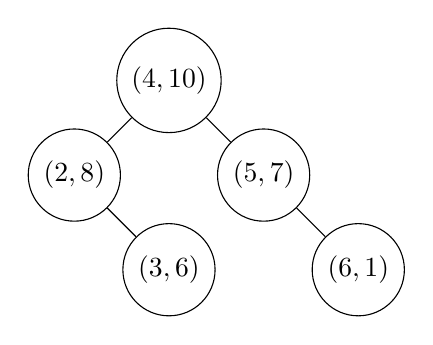
\begin{tikzpicture}[node distance = 1.7cm]
    \node[state] (A) {$(4, 10)$};
    \node[state] (B) [below left of=A] {$(2, 8)$};
    \node[state] (C) [below right of=B] {$(3, 6)$};
    \node[state] (D) [below right of=A] {$(5, 7)$};
    \node[state] (E) [below right of=D] {$(6, 1)$};
    \path (A) edge (B)
          (B) edge (C)
          (A) edge (D)
          (D) edge (E);
  \end{tikzpicture}
  \quad\quad
  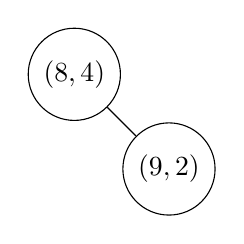
\begin{tikzpicture}[node distance = 1.7cm]
    \node[state] (A) {$(8, 4)$};
    \node[state] (B) [below right of=A] {$(9, 2)$};
    \path (A) edge (B);
  \end{tikzpicture}
  \caption{Example of Split with a threshold of 7.}
\end{figure}

The operation \textbf{merge} is the reverse operation. We take two treaps as input, assuming that the values of the first coordinates of the nodes of the first treap are lower than the one of the second treap, and we merge them to get back the initial treap.

\medskip We can now give a small pseudo-code for those two operations. It is very easy to write such a code in a functional language.

\begin{verbatim}
Function merge(treap A, treap B):
  If A is empty: return B
  If B is empty: return A
  If A.heap > B.heap:
    A.right = merge(A.right, B)
    return A
  else:
    B.left = merge(A, B.left)
    return B
\end{verbatim}

\begin{verbatim}
Function split(treap T, threshold X):
  If T is empty: return T
  If T.bst <= X:
    A, T.left = split(T.left, X)
    return A, T
  else:
    T.right, B = split(A, B.left)
    return T, B
\end{verbatim}

The amortized complexity of those operations is in $\mathcal O(\log N)$ where $N$ is the number of nodes. Indeed if we sample the value \verb|heap| randomly, the tree is balanced.

\newpage
\subsection{Applications}

Now that we have implemented operations \verb|split| and \verb|merge|, we can easily deduce operations \verb|insert| and \verb|remove|.

\begin{verbatim}
Function insert(treap T, node N):
  A, B = split(T, N.bst)
  return merge(A, merge(N, B))
\end{verbatim} 

\begin{verbatim}
Function remove(treap T, value X):
  A, B = split(T, X)
  _, C = split(B, X+1)
  return merge(A, C)
\end{verbatim} 

We can now notice that with the assumption on the input of the merge function, values of the \textbf{first coordinate} (BST) of each node could be implicit. Indeed the structure of the tree imposes an order (infix) on the nodes. So we could replace it by the \textbf{size of the subtree} (updated after during each operation). The split threshold now becomes the rank of the value for which the cut is done.

\medskip This data-structure is very easy to implement in a classical language of programmation. In the next part we are going to explain how we managed to implement it in Erlang, each node of the tree being handled by a different process.

\newpage

\section{Middle-ware}

\subsection{Global overview}

The organization of the project is the following. Source files are stored in the \verb|src| directory. The \verb|Makefile| can be used for the compilation and agent deployment. The python script \verb|slsu.py| can be use to extract hostnames from \verb|.hosts.erlang| and launch an agent on each of those nodes.

\begin{verbatim}
+-- bin
|   +-- .hosts.erlang
|   +-- compiled files...
+-- src
|   +-- agent.erl
|   +-- jobs.erl
|   +-- monitor.erl
+-- Makefile
+-- slsu.py
\end{verbatim}

\noindent The file \verb|agent.erl| contains all the internal functions used by the agents. We can describe an agent by a finite state machine. 


\begin{figure}[h!]
  \centering
  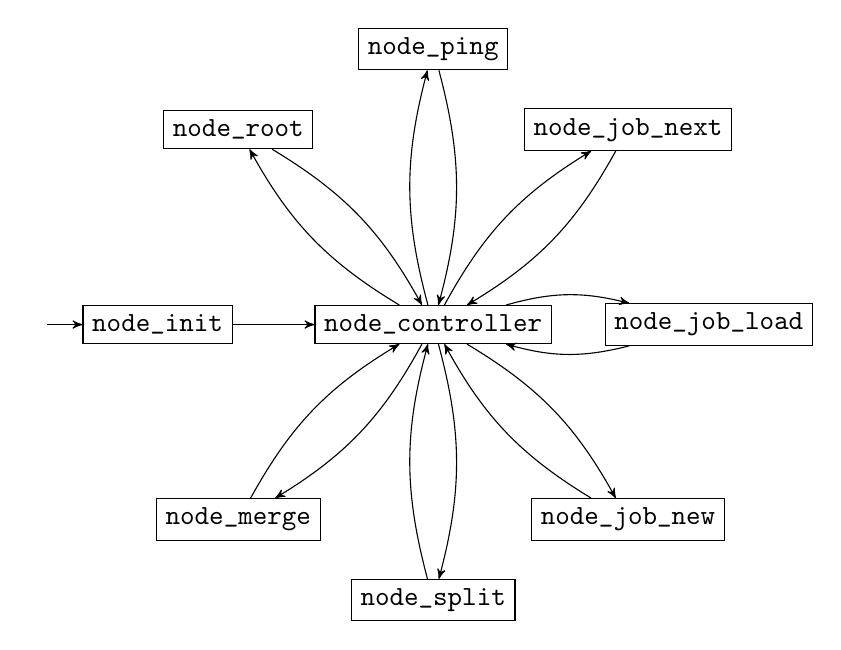
\begin{tikzpicture}[node distance = 3.5cm, ->, >=stealth', bend angle=15, initial text={}]
    \tikzset{state/.style={draw,rectangle}}
    \node[initial,state] (init) {\verb|node_init|};
    \node[state] (controller) [right of=init]             {\verb|node_controller|};
    \node[state] (root)       [above left of=controller]  {\verb|node_root|};
    \node[state] (ping)       [above of=controller]       {\verb|node_ping|};
    \node[state] (job_next)   [above right of=controller] {\verb|node_job_next|};
    \node[state] (job_load)   [right of=controller]       {\verb|node_job_load|};
    \node[state] (job_new)    [below right of=controller] {\verb|node_job_new|};
    \node[state] (split)      [below of=controller]       {\verb|node_split|};
    \node[state] (merge)      [below left of=controller]  {\verb|node_merge|};
    \path (controller) edge [bend left] (root)
          (root)       edge [bend left] (controller)
          (controller) edge [bend left] (ping)
          (ping)       edge [bend left] (controller)
          (controller) edge [bend left] (job_next)
          (job_next)   edge [bend left] (controller)
          (controller) edge [bend left] (job_new)
          (job_new)    edge [bend left] (controller)
          (controller) edge [bend left] (job_load)
          (job_load)   edge [bend left] (controller)
          (controller) edge [bend left] (split)
          (split)      edge [bend left] (controller)
          (controller) edge [bend left] (merge)
          (merge)      edge [bend left] (controller)
          (init)       edge             (controller);
  \end{tikzpicture}
  \caption{Finite State Machine describing an Agent.}
\end{figure}

\begin{itemize}
	\item \verb|node_init| is the initialization state. 
	\item \verb|node_controller| receives messages. It branch toward the state that handle the message that has just been received
	\item \verb|node_root| send a message to the father of the node in order to return the root of the topoogy.
	\item \verb|node_ping| sequentially send a message to the left child then to the right child in order to return a list of all the nodes of the topology (in postfix order)
	\item \verb|node_job_next| is the function responsible to spawn a new process if a new job is received or if a job token is released.
	\item \verb|node_job_load| is responsible to update upward the load value of the nodes. When one node finishes the execution of one job, the load value of its ancestors is updated
	\item \verb|node_job_new| search for the best node on which execute a new job, taking into account the current load of each node of the topology.
	\item \verb|node_split| handles the split operation.
	\item \verb|node_merge| handles the merge operation.
\end{itemize}

\noindent The file \verb|monitor.erl| implements several interface function to manipulate the treap topology.
\begin{itemize}
	\item \verb|ask_merge(RootTreap1, RootTreap2)| merges two treaps.
	\item \verb|ask_split(RootTreap, Rank)| split the treap according to the threshold. It returns two treaps, the first one having a size \verb|Rank| (if the threshold was valid).
	\item \verb|ask_remove(RootTreap, Rank)| kills the process of rank \verb|Rank| and maintains a coherent topology.
	\item \verb|ask_root(NodeTreap)| returns the identifier of the root of the treap in which \verb|NodeTreap| is.
	\item \verb|ask_ping(RootTreap)| returns the list of all the identifiers of the nodes of the treap rooted in \verb|RootTreap|.
	\item \verb|ask_job(RootTreap, Mod, Fun, Args)| submit one job in the topology. The process that called this function must expect to receive the return value of the job. As nodes at the top of the treap may forward a lot of jobs, a node can accept a job only if the size of its subtree is lower than a given threshold.
	\item \verb|ask_kill(RootTreap)| kills all the nodes of the treap.
	\item \verb|ask_graph(RootTreap, Filename)| exports a graph representing the topology (graphviz dot format)
	\item \verb|ask_say_hello(RootTreap)| ask each node of the treap to say hello!
\end{itemize}

\subsection{Results}

\subsubsection{Complexity}

The complexity of the requests \verb|ask_ping|, \verb|ask_graph| and \verb|ask_kill| is linear in the size of the treap (the tree is traveled sequentially).
The amortized complexity of all the other operations is logarithmic in the size of the treap.

One particular case is when we perform several merge request consecutively. When the merging process is finished on one node and continues with one of its children, a new merge request can be started. The complexity of performing $N$ merge request on a treap of size $M$ is therefore $\mathcal O(N + \log M)$. It is also true when submitting $N$ jobs to a treap of size $M$.

The amortized complexity to add one node to the topology or to submit one job is therefore constant.

\subsubsection{Graphs}

Here is an example of a graph we get when running our topology on 14 nodes of the SLSU cluster (using \verb|slsu.py| and \verb|monitor:ask_graph|).

\begin{figure}[h!]
\centering
\includegraphics[width=11cm]{graph.pdf}
\caption{Example of Graph}
\end{figure}

\newpage

\subsection{Questions answered}

Here is a quick summary of what we have implemented regarding to the questions asked in the project assignment.

\paragraph{Agent deployment}
\begin{enumerate}[label=\alph*)]
	\item Spawn an agent that wait for a remote command: \verb|spawn(agent, node_init, [1])|.
	\item Have this agent part of a coherent topology: \verb|monitor:ask_merge/2|.
	\item Be able to have a new agent join an existing topoogy: \verb|monitor:ask_merge/2|.
	\item Have the possibility to remotely kill an agent: \verb|monitor:ask_remove/2|.
\end{enumerate}

\paragraph{Job execution}

\begin{enumerate}[label=\alph*)]
  \item Be able to receive job request and send back the results: \verb|agent:node_job_next|.
  \item Keep a waiting list (see \verb|treap.jobs|) so that no more than one job is performed simultaneously on this specific node (the argument of \verb|agent:node_init/1| is the number of job tokens).
  \item Have a voting that selects where to execute the job: \verb|agent:node_job_new|.
\end{enumerate}

\paragraph{Agent monitoring}
\begin{enumerate}[label=\alph*)]
	\item Given an hostname, remotely spawn an agent on that node and have it join the topology: see installation instructions, either manually with the makefile or automatically using the python script.
	\item Query the topology for statistics: \verb|monitor:ask_ping/1| and \verb|monitor:ask_graph/2|.
	\item Submit job to one specific node: not implemented because of d), but easy with two splits, one job request and two merges. 
	\item Submit job to be executed on any node: \verb|monitor:ask_job/4|.
	\item Build a script that, given a set of nodes, automatically deploy the platform so that it is ready to accept new jobs: \verb|slsu.py|.
\end{enumerate}

\paragraph{Going further}
\begin{enumerate}[label=\alph*)]
  \item Have multiple monitors: just run \verb|make monitor| twice.
  \item[d)] Merge and Split operations are useful if we want to use our middle-ware with several kinds of jobs (some time consuming jobs and a lot of fast jobs). Our voting process considers that jobs are all similar. If it is not the case, you can just split the network in two!
\end{enumerate}

\newpage

\section{Installation}

\subsection{Using python script}

Fill the hosts file (\verb|bin/.hosts.erlang|) with the name of the servers you want to use as nodes. Make sure that you can access those nodes using ssh without password (e.g. public key authorized). Then run the python script \verb|slsu.py|.

\subsection{Create agents}

On each machine, run \verb|make agent|.

\medskip\noindent You can rename the node using for example \verb|make NAME=node@192.168.0.1|.

\medskip\noindent If you want to run two independant instances of the middleware at the same time, you can change the cookie of the erlang nodes with \verb|make COOKIE=seed|. To nodes will be able to connect to one other if and only if their cookies are identical.

\subsection{Create hosts file}

Update the hosts file (\verb|bin/.hosts.erlang|) using to the following syntax.
\begin{verbatim}
'192.168.0.1'.
'192.168.0.2'.
\end{verbatim}

One possible error is that the agents you deployed don't answer to request if their name is the default one or because of the DNS server. If it happens, please use IP adresses and rename the agents.

\subsection{Launch the monitor}

Finally you can merge the agents you just deployed in a coherent topology. The hosts file must be on the computer on which you we run \verb|make monitor|.

\medskip\noindent You can now have fun with erlang's shell !
\begin{verbatim}
nodes().
Pid = global:whereis_name(agent).
monitor:ask_graph(Pid, "graph.dot").
monitor:ask_job(Pid, jobs, wait, [2000]).
receive ok -> ok end.
monitor:stop().
\end{verbatim}


\end{document}